\chapter{Introdução Teórica}

Não é possível entrar no tema \textbf{Meio Ambiente} sem mencionar a Educação Ambiental nas escolas, uma vez que esperamos que nossas crianças evoluam com uma mentalidade melhor que a nossa no tocante ao meio ambiente.\\

\citeaa{Dias1994}  diz que a "Educação Ambiental se caracteriza por
incorporar as dimensões sociais, políticas, econômicas,
culturais, ecológicas e éticas, deixando claro que ao discutir
qualquer problema ambiental é fundamental a consideração
de todos estes aspectos." Segundo este autor, "a maior parte
dos problemas ambientais tem suas raízes na miséria que,
por sua vez, é gerada por políticas e problemas econômicos,
concentradores de riqueza e responsáveis pelo desemprego
e degradação ambiental."\\

Pode-se também definir a educação ambiental, nas palavras de \citeonline{Magalhaes2018}, como um processo
onde o educando obtém conhecimentos acerca das
questões ambientais e assim passa a ter um novo
entendimento acerca do meio ambiente, se tornando um
agente transformador referente à preservação do meio
ambiente e de seus recursos naturais. \\

\citeaa{Gadotti2000} explica que educação ambiental vai muito além do conservacionismo
Trata-se de uma mudança radical de mentalidade em
relação à qualidade de vida, que está diretamente ligada
ao tipo de convivência que mantemos com a natureza e
que implica em atitudes, valores, ações. Trata-se de uma
opção de vida por uma relação saudável e equilibrada,
com o contexto, com os outros, com o ambiente mais
próximo, a começar pelo ambiente de trabalho e
doméstico.\\

\section{Contexto Geográfico: Brasília}

De acordo com dados da \citeaa{WikiPediaBrasilia20200518} A cidade começou a ser planejada e desenvolvida em 1956 por Lúcio Costa, pelo também arquiteto Oscar Niemeyer e pelo engenheiro estrutural Joaquim Cardozo. Inaugurada em 21 de abril de 1960, pelo então presidente Juscelino Kubitschek, Brasília tornou-se formalmente a terceira capital do Brasil, após Salvador e Rio de Janeiro. Vista de cima, a principal área da cidade é descrita frequentemente como tendo o formato de um avião, mas a proposta inicial de Lúcio Costa era de que se assemelhasse ao sinal da cruz, e um dos eixos foi depois arqueado para se adaptar ao relevo da região.\\

O ritmo de crescimento populacional na primeira década foi de 14,4\% ao ano, com um aumento populacional de 285\%. Na década de 1970, o crescimento médio anual foi de 8,1\%, com um incremento total de 115,52\%. A população total do Distrito Federal, que não deveria ultrapassar 500 000 habitantes em 2000, atingiu esta cota no início da década de 1970, e, entre 1980 e 1991, a população expandiu em mais 32,8\%. O Plano Piloto, que, na inauguração, concentrava 48\% da população do Distrito Federal, gradativamente perdeu importância relativa, chegando a 13,26\% em 1991, passando o predomínio para as cidades-satélite.

Em 2010, o Instituto Brasileiro de Geografia e Estatística indicou 2.570.160 habitantes em todo o Distrito Federal. O Índice de Desenvolvimento Humano é de 0,824 e a taxa de analfabetismo de apenas 4,35\%. Brasília também caracteriza-se pela sua desigualdade social, sendo a quarta área metropolitana mais desigual do Brasil e a décima sexta do mundo, segundo um relatório divulgado pela Organização das Nações Unidas. \\

A população brasiliense é formada por migrantes de todas as regiões brasileiras, sobretudo do Nordeste e do Sudeste, além de estrangeiros que trabalham nas embaixadas espalhadas pela capital. Dados de 2010 apontavam que quase metade da população não nasceu ali, sendo que 1.380.873 (53,73\%) eram brasilienses e 1.189.287 (46,27\%) de outros locais (incluindo 8.577 estrangeiros, ou 0,33\% da população), principalmente de Goiás, Minas Gerais e Bahia.\\

Esse dado é reforçado pelos dados da \citeaa{CODEPLANSEPLAN2013}. Nos quadros abaixo mostram a composição da população migrante de brasília:


\begin{figure}[h!]
    \centering
    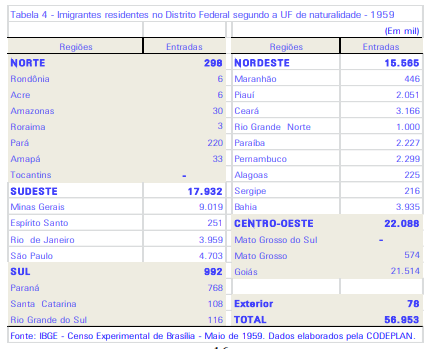
\includegraphics{fig/imigrantes-1959}
    \label{table:imigrantes-1959}
    \caption{Imigrantes residentes no DF em 1959}
\end{figure}

\begin{figure}[h!]
    \centering
    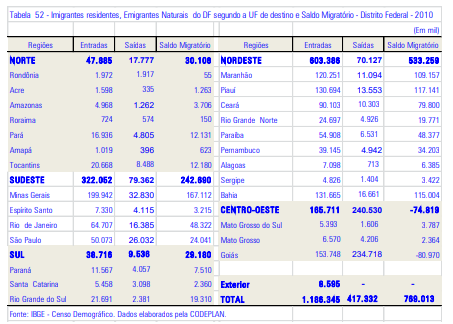
\includegraphics{fig/imigrantes-2010}
    \caption{Imigrantes residentes no DF em 2010}
    \label{table:imigrantes-2010}
\end{figure}


Ainda de acordo com \citeaa{WikiPediaBrasilia20200518}, a região administrativa de Brasília, composta em sua parte urbana pelos bairros residenciais Asa Norte, Asa Sul e Vila Planalto, conta com uma população de 209 855 habitantes (2010) e uma área de 472,12 km², sendo a terceira maior região administrativa do Distrito Federal em termos de população, atrás apenas de Ceilândia (com 402.729 habitantes) e Taguatinga (361.063).\\

Brasília possui a maior desigualdade de renda entre as capitais brasileiras, além de ser uma das capitais em que mais se registram homicídios para cada cem mil habitantes no país. Na região administrativa de Ceilândia, está localizada a segunda mais populosa favela do Brasil, a comunidade do Sol Nascente, com 61 mil habitantes — segundo estimativas de lideranças locais, no entanto, a população seria de 100 mil pessoas, que superaria a da Rocinha, no Rio de Janeiro.\\

Note no mapa abaixo que as áreas em cinza são zonas "sem dados" são principalmente regiões administrativas novas, a maioria contem a maioria dos habitantes mais pobres do distrito federal\\

A tabela abaixo descreve o IDH das regiões administratívas do Distrito Federal.\\


\begin{figure}[h!]
    \centering
    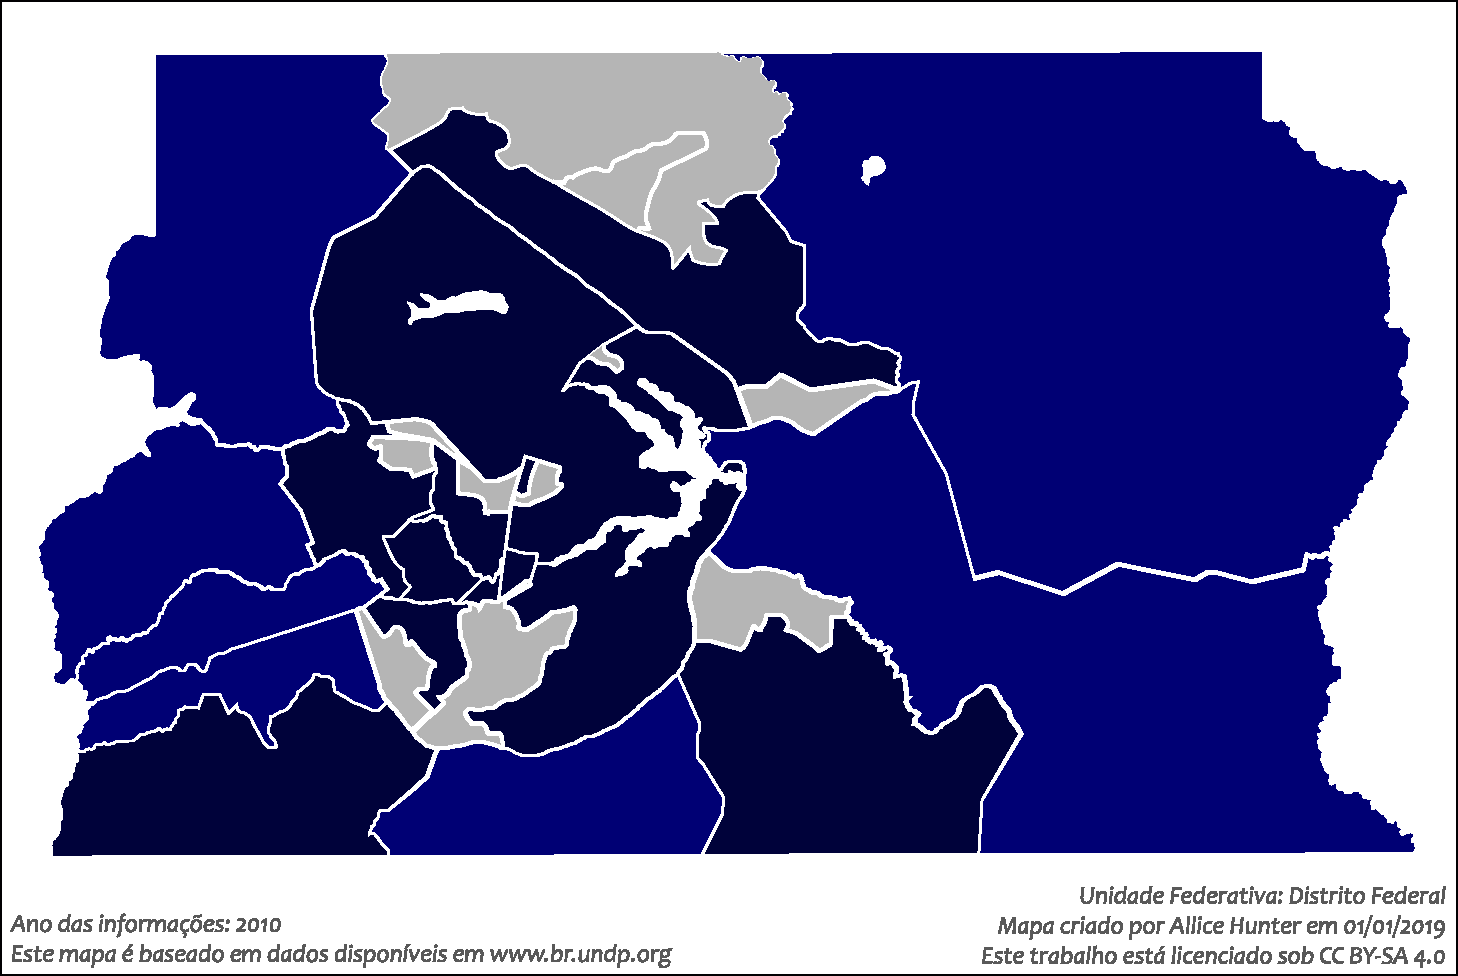
\includegraphics[width=0.6\linewidth]{2-caps/cap02/Mapa_do_IDH_do_Distrito_Federal_(2010)}
    \caption{Mapa do Distrito Federal separada por regiões administrativas.}
    \label{fig:mapadoidhdodistritofederal2010}
\end{figure}

% Please add the following required packages to your document preamble:
% \usepackage{multirow}
% \usepackage[table,xcdraw]{xcolor}
% If you use beamer only pass "xcolor=table" option, i.e. \documentclass[xcolor=table]{beamer}
\begin{center}
    \begin{table}[]
        \centering
        \resizebox{.5\textwidth}{!}{
            \begin{tabular}{llllll}
                \rowcolor[HTML]{EAECF0}
                \multicolumn{1}{c}{\cellcolor[HTML]{EAECF0}{\color[HTML]{202122} }} &
                \multicolumn{1}{c}{\cellcolor[HTML]{EAECF0}{\color[HTML]{202122} }} &
                \multicolumn{4}{c}{\cellcolor[HTML]{EAECF0}{\color[HTML]{202122} \textbf{Dados de 2010}}} \\
                \rowcolor[HTML]{EAECF0}
                \multicolumn{1}{c}{\multirow{-2}{*}{\cellcolor[HTML]{EAECF0}{\color[HTML]{202122} \textbf{Posição}}}} &
                \multicolumn{1}{c}{\multirow{-2}{*}{\cellcolor[HTML]{EAECF0}{\color[HTML]{202122} \textbf{Região administrativa}}}} &
                \multicolumn{1}{c}{\cellcolor[HTML]{EAECF0}{\color[HTML]{0B0080} \textbf{IDH-M}}} &
                \multicolumn{1}{c}{\cellcolor[HTML]{EAECF0}{\color[HTML]{202122} \textbf{IDH-R}}} &
                \multicolumn{1}{c}{\cellcolor[HTML]{EAECF0}{\color[HTML]{202122} \textbf{IDH-L}}} &
                \multicolumn{1}{c}{\cellcolor[HTML]{EAECF0}{\color[HTML]{202122} \textbf{IDH-E}}} \\
                \rowcolor[HTML]{EAECF0}
                \cellcolor[HTML]{00023A}{\color[HTML]{0000FF} \textbf{}} &
                \multicolumn{5}{l}{\cellcolor[HTML]{EAECF0}{\color[HTML]{00023A} \textbf{IDH-M muito alto}}} \\
                \rowcolor[HTML]{F8F9FA}
                {\color[HTML]{202122} 1} &
                {\color[HTML]{0B0080} Águas Claras} &
                {\color[HTML]{202122} \textbf{0,955}} &
                {\color[HTML]{202122} 1,000} &
                {\color[HTML]{202122} 0,934} &
                {\color[HTML]{202122} 0,936} \\
                \rowcolor[HTML]{F8F9FA}
                {\color[HTML]{202122} 2} &
                {\color[HTML]{0B0080} Lago Sul} &
                {\color[HTML]{202122} \textbf{0,955}} &
                {\color[HTML]{202122} 1,000} &
                {\color[HTML]{202122} 0,953} &
                {\color[HTML]{202122} 0,915} \\
                \rowcolor[HTML]{F8F9FA}
                {\color[HTML]{202122} 3} &
                {\color[HTML]{0B0080} Plano Piloto} &
                {\color[HTML]{202122} \textbf{0,936}} &
                {\color[HTML]{202122} 0,948} &
                {\color[HTML]{202122} 0,870} &
                {\color[HTML]{202122} 0,991} \\
                \rowcolor[HTML]{F8F9FA}
                {\color[HTML]{202122} 4} &
                {\color[HTML]{0B0080} Lago Norte} &
                {\color[HTML]{202122} \textbf{0,933}} &
                {\color[HTML]{202122} 0,978} &
                {\color[HTML]{202122} 0,864} &
                {\color[HTML]{202122} 0,958} \\
                \rowcolor[HTML]{F8F9FA}
                {\color[HTML]{202122} 5} &
                {\color[HTML]{0B0080} Cruzeiro} &
                {\color[HTML]{202122} \textbf{0,928}} &
                {\color[HTML]{202122} 0,934} &
                {\color[HTML]{202122} 0,857} &
                {\color[HTML]{202122} 0,992} \\
                \rowcolor[HTML]{F8F9FA}
                {\color[HTML]{202122} 6} &
                {\color[HTML]{0B0080} Núcleo Bandeirante} &
                {\color[HTML]{202122} \textbf{0,911}} &
                {\color[HTML]{202122} 0,934} &
                {\color[HTML]{202122} 0,811} &
                {\color[HTML]{202122} 0,988} \\
                \rowcolor[HTML]{F8F9FA}
                {\color[HTML]{202122} 7} &
                {\color[HTML]{0B0080} Guará} &
                {\color[HTML]{202122} \textbf{0,867}} &
                {\color[HTML]{202122} 0,831} &
                {\color[HTML]{202122} 0,826} &
                {\color[HTML]{202122} 0,944} \\
                \rowcolor[HTML]{F8F9FA}
                {\color[HTML]{202122} 8} &
                {\color[HTML]{0B0080} Taguatinga} &
                {\color[HTML]{202122} \textbf{0,855}} &
                {\color[HTML]{202122} 0,806} &
                {\color[HTML]{202122} 0,816} &
                {\color[HTML]{202122} 0,944} \\
                \rowcolor[HTML]{F8F9FA}
                {\color[HTML]{202122} 9} &
                {\color[HTML]{0B0080} Candangolândia} &
                {\color[HTML]{202122} \textbf{0,852}} &
                {\color[HTML]{202122} 0,761} &
                {\color[HTML]{202122} 0,850} &
                {\color[HTML]{202122} 0,947} \\
                \rowcolor[HTML]{F8F9FA}
                {\color[HTML]{202122} 10} &
                {\color[HTML]{0B0080} Sobradinho} &
                {\color[HTML]{202122} \textbf{0,837}} &
                {\color[HTML]{202122} 0,763} &
                {\color[HTML]{202122} 0,825} &
                {\color[HTML]{202122} 0,923} \\
                \rowcolor[HTML]{F8F9FA}
                {\color[HTML]{202122} 11} &
                {\color[HTML]{0B0080} Riacho Fundo} &
                {\color[HTML]{202122} \textbf{0,826}} &
                {\color[HTML]{202122} 0,706} &
                {\color[HTML]{202122} 0,815} &
                {\color[HTML]{202122} 0,958} \\
                \rowcolor[HTML]{F8F9FA}
                {\color[HTML]{202122} 12} &
                {\color[HTML]{0B0080} São Sebastião} &
                {\color[HTML]{202122} \textbf{0,820}} &
                {\color[HTML]{202122} 0,714} &
                {\color[HTML]{202122} 0,804} &
                {\color[HTML]{202122} 0,944} \\
                \rowcolor[HTML]{F8F9FA}
                {\color[HTML]{202122} 13} &
                {\color[HTML]{0B0080} Gama} &
                {\color[HTML]{202122} \textbf{0,815}} &
                {\color[HTML]{202122} 0,720} &
                {\color[HTML]{202122} 0,784} &
                {\color[HTML]{202122} 0,942} \\
                \rowcolor[HTML]{EAECF0}
                \cellcolor[HTML]{000074}{\color[HTML]{009900} \textbf{}} &
                \multicolumn{5}{l}{\cellcolor[HTML]{EAECF0}{\color[HTML]{000074} \textbf{IDH-M alto}}} \\
                \rowcolor[HTML]{F8F9FA}
                {\color[HTML]{202122} 14} &
                {\color[HTML]{0B0080} Santa Maria} &
                {\color[HTML]{202122} \textbf{0,794}} &
                {\color[HTML]{202122} 0,627} &
                {\color[HTML]{202122} 0,820} &
                {\color[HTML]{202122} 0,934} \\
                \rowcolor[HTML]{F8F9FA}
                {\color[HTML]{202122} 15} &
                {\color[HTML]{0B0080} Paranoá} &
                {\color[HTML]{202122} \textbf{0,785}} &
                {\color[HTML]{202122} 0,612} &
                {\color[HTML]{202122} 0,800} &
                {\color[HTML]{202122} 0,948} \\
                \rowcolor[HTML]{F8F9FA}
                {\color[HTML]{202122} 16} &
                {\color[HTML]{0B0080} Ceilândia} &
                {\color[HTML]{202122} \textbf{0,784}} &
                {\color[HTML]{202122} 0,670} &
                {\color[HTML]{202122} 0,773} &
                {\color[HTML]{202122} 0,910} \\
                \rowcolor[HTML]{F8F9FA}
                {\color[HTML]{202122} 17} &
                {\color[HTML]{0B0080} Samambaia} &
                {\color[HTML]{202122} \textbf{0,781}} &
                {\color[HTML]{202122} 0,629} &
                {\color[HTML]{202122} 0,791} &
                {\color[HTML]{202122} 0,921} \\
                \rowcolor[HTML]{F8F9FA}
                {\color[HTML]{202122} 18} &
                {\color[HTML]{0B0080} Recanto das Emas} &
                {\color[HTML]{202122} \textbf{0,775}} &
                {\color[HTML]{202122} 0,598} &
                {\color[HTML]{202122} 0,791} &
                {\color[HTML]{202122} 0,937} \\
                \rowcolor[HTML]{F8F9FA}
                {\color[HTML]{202122} 19} &
                {\color[HTML]{0B0080} Planaltina} &
                {\color[HTML]{202122} \textbf{0,764}} &
                {\color[HTML]{202122} 0,652} &
                {\color[HTML]{202122} 0,769} &
                {\color[HTML]{202122} 0,872} \\
                \rowcolor[HTML]{F8F9FA}
                {\color[HTML]{202122} 20} &
                {\color[HTML]{0B0080} Brazlândia} &
                {\color[HTML]{202122} \textbf{0,761}} &
                {\color[HTML]{202122} 0,642} &
                {\color[HTML]{202122} 0,734} &
                {\color[HTML]{202122} 0,906} \\
                \rowcolor[HTML]{FFFFFF}
                \multicolumn{1}{c}{\cellcolor[HTML]{B5B5B5}{\color[HTML]{202122} \textbf{}}} &
                \multicolumn{5}{l}{\cellcolor[HTML]{FFFFFF}{\color[HTML]{656565} \textbf{Sem dados}}} \\
                \rowcolor[HTML]{F8F9FA}
                \multicolumn{6}{c}{\cellcolor[HTML]{F8F9FA}{\color[HTML]{0B0080} Sudoeste/Octogonal}} \\
                \rowcolor[HTML]{F8F9FA}
                \multicolumn{6}{c}{\cellcolor[HTML]{F8F9FA}{\color[HTML]{0B0080} Varjão}} \\
                \rowcolor[HTML]{F8F9FA}
                \multicolumn{6}{c}{\cellcolor[HTML]{F8F9FA}{\color[HTML]{0B0080} Park Way}} \\
                \rowcolor[HTML]{F8F9FA}
                \multicolumn{6}{c}{\cellcolor[HTML]{F8F9FA}{\color[HTML]{0B0080} Riacho Fundo II}} \\
                \rowcolor[HTML]{F8F9FA}
                \multicolumn{6}{c}{\cellcolor[HTML]{F8F9FA}{\color[HTML]{0B0080} SCIA}} \\
                \rowcolor[HTML]{F8F9FA}
                \multicolumn{6}{c}{\cellcolor[HTML]{F8F9FA}{\color[HTML]{0B0080} Sobradinho II}} \\
                \rowcolor[HTML]{F8F9FA}
                \multicolumn{6}{c}{\cellcolor[HTML]{F8F9FA}{\color[HTML]{0B0080} Jardim Botânico}} \\
                \rowcolor[HTML]{F8F9FA}
                \multicolumn{6}{c}{\cellcolor[HTML]{F8F9FA}{\color[HTML]{0B0080} Itapoã}} \\
                \rowcolor[HTML]{F8F9FA}
                \multicolumn{6}{c}{\cellcolor[HTML]{F8F9FA}{\color[HTML]{0B0080} SIA}} \\
                \rowcolor[HTML]{F8F9FA}
                \multicolumn{6}{c}{\cellcolor[HTML]{F8F9FA}{\color[HTML]{0B0080} Vicente Pires}} \\
                \rowcolor[HTML]{F8F9FA}
                \multicolumn{6}{c}{\cellcolor[HTML]{F8F9FA}{\color[HTML]{0B0080} Fercal}}
            \end{tabular}
        }
        \caption{IDH das Regiões Administrativas de Brasília.\\ O IDH-M é uma média geométrica entre o IDH da renda (IDH-R), IDH da longevidade (IDH-L) e IDH educacional (IDH-E).}
        \label{table:IDH}
    \end{table}
\end{center}

Ao observar

Os índices de criminalidade são altos principalmente no Entorno do Distrito Federal. Segundo sociólogos, a criminalidade no Distrito Federal, principalmente nas cidades-satélites, é uma herança do crescimento desordenado, ainda que assentado em núcleos urbanos planejados. Os níveis de criminalidade no DF estão entre os maiores do Brasil, chegando ao ponto de haver uma média de até dois assassinatos diários. Em 2012, houve 1031 homicídios, com taxa de 38,9 por 100 mil habitantes, a 478º maior do país. Existem diversas propostas para tentar diminuir a criminalidade na capital: entre elas, um maior policiamento, medida esta que, aplicada, tem levado a uma retração da violência.\\


%\newacronym{CODEPLAN}{CODEPLAN}{Companhia de Planejamento do Distrito Federal}

